% Options for packages loaded elsewhere
\PassOptionsToPackage{unicode}{hyperref}
\PassOptionsToPackage{hyphens}{url}
\PassOptionsToPackage{dvipsnames,svgnames,x11names}{xcolor}
%
\documentclass[
  authoryear]{elsarticle}

\usepackage{amsmath,amssymb}
\usepackage{iftex}
\ifPDFTeX
  \usepackage[T1]{fontenc}
  \usepackage[utf8]{inputenc}
  \usepackage{textcomp} % provide euro and other symbols
\else % if luatex or xetex
  \usepackage{unicode-math}
  \defaultfontfeatures{Scale=MatchLowercase}
  \defaultfontfeatures[\rmfamily]{Ligatures=TeX,Scale=1}
\fi
\usepackage{lmodern}
\ifPDFTeX\else  
    % xetex/luatex font selection
\fi
% Use upquote if available, for straight quotes in verbatim environments
\IfFileExists{upquote.sty}{\usepackage{upquote}}{}
\IfFileExists{microtype.sty}{% use microtype if available
  \usepackage[]{microtype}
  \UseMicrotypeSet[protrusion]{basicmath} % disable protrusion for tt fonts
}{}
\makeatletter
\@ifundefined{KOMAClassName}{% if non-KOMA class
  \IfFileExists{parskip.sty}{%
    \usepackage{parskip}
  }{% else
    \setlength{\parindent}{0pt}
    \setlength{\parskip}{6pt plus 2pt minus 1pt}}
}{% if KOMA class
  \KOMAoptions{parskip=half}}
\makeatother
\usepackage{xcolor}
\setlength{\emergencystretch}{3em} % prevent overfull lines
\setcounter{secnumdepth}{2}
% Make \paragraph and \subparagraph free-standing
\ifx\paragraph\undefined\else
  \let\oldparagraph\paragraph
  \renewcommand{\paragraph}[1]{\oldparagraph{#1}\mbox{}}
\fi
\ifx\subparagraph\undefined\else
  \let\oldsubparagraph\subparagraph
  \renewcommand{\subparagraph}[1]{\oldsubparagraph{#1}\mbox{}}
\fi

\usepackage{color}
\usepackage{fancyvrb}
\newcommand{\VerbBar}{|}
\newcommand{\VERB}{\Verb[commandchars=\\\{\}]}
\DefineVerbatimEnvironment{Highlighting}{Verbatim}{commandchars=\\\{\}}
% Add ',fontsize=\small' for more characters per line
\usepackage{framed}
\definecolor{shadecolor}{RGB}{241,243,245}
\newenvironment{Shaded}{\begin{snugshade}}{\end{snugshade}}
\newcommand{\AlertTok}[1]{\textcolor[rgb]{0.68,0.00,0.00}{#1}}
\newcommand{\AnnotationTok}[1]{\textcolor[rgb]{0.37,0.37,0.37}{#1}}
\newcommand{\AttributeTok}[1]{\textcolor[rgb]{0.40,0.45,0.13}{#1}}
\newcommand{\BaseNTok}[1]{\textcolor[rgb]{0.68,0.00,0.00}{#1}}
\newcommand{\BuiltInTok}[1]{\textcolor[rgb]{0.00,0.23,0.31}{#1}}
\newcommand{\CharTok}[1]{\textcolor[rgb]{0.13,0.47,0.30}{#1}}
\newcommand{\CommentTok}[1]{\textcolor[rgb]{0.37,0.37,0.37}{#1}}
\newcommand{\CommentVarTok}[1]{\textcolor[rgb]{0.37,0.37,0.37}{\textit{#1}}}
\newcommand{\ConstantTok}[1]{\textcolor[rgb]{0.56,0.35,0.01}{#1}}
\newcommand{\ControlFlowTok}[1]{\textcolor[rgb]{0.00,0.23,0.31}{\textbf{#1}}}
\newcommand{\DataTypeTok}[1]{\textcolor[rgb]{0.68,0.00,0.00}{#1}}
\newcommand{\DecValTok}[1]{\textcolor[rgb]{0.68,0.00,0.00}{#1}}
\newcommand{\DocumentationTok}[1]{\textcolor[rgb]{0.37,0.37,0.37}{\textit{#1}}}
\newcommand{\ErrorTok}[1]{\textcolor[rgb]{0.68,0.00,0.00}{#1}}
\newcommand{\ExtensionTok}[1]{\textcolor[rgb]{0.00,0.23,0.31}{#1}}
\newcommand{\FloatTok}[1]{\textcolor[rgb]{0.68,0.00,0.00}{#1}}
\newcommand{\FunctionTok}[1]{\textcolor[rgb]{0.28,0.35,0.67}{#1}}
\newcommand{\ImportTok}[1]{\textcolor[rgb]{0.00,0.46,0.62}{#1}}
\newcommand{\InformationTok}[1]{\textcolor[rgb]{0.37,0.37,0.37}{#1}}
\newcommand{\KeywordTok}[1]{\textcolor[rgb]{0.00,0.23,0.31}{\textbf{#1}}}
\newcommand{\NormalTok}[1]{\textcolor[rgb]{0.00,0.23,0.31}{#1}}
\newcommand{\OperatorTok}[1]{\textcolor[rgb]{0.37,0.37,0.37}{#1}}
\newcommand{\OtherTok}[1]{\textcolor[rgb]{0.00,0.23,0.31}{#1}}
\newcommand{\PreprocessorTok}[1]{\textcolor[rgb]{0.68,0.00,0.00}{#1}}
\newcommand{\RegionMarkerTok}[1]{\textcolor[rgb]{0.00,0.23,0.31}{#1}}
\newcommand{\SpecialCharTok}[1]{\textcolor[rgb]{0.37,0.37,0.37}{#1}}
\newcommand{\SpecialStringTok}[1]{\textcolor[rgb]{0.13,0.47,0.30}{#1}}
\newcommand{\StringTok}[1]{\textcolor[rgb]{0.13,0.47,0.30}{#1}}
\newcommand{\VariableTok}[1]{\textcolor[rgb]{0.07,0.07,0.07}{#1}}
\newcommand{\VerbatimStringTok}[1]{\textcolor[rgb]{0.13,0.47,0.30}{#1}}
\newcommand{\WarningTok}[1]{\textcolor[rgb]{0.37,0.37,0.37}{\textit{#1}}}

\providecommand{\tightlist}{%
  \setlength{\itemsep}{0pt}\setlength{\parskip}{0pt}}\usepackage{longtable,booktabs,array}
\usepackage{calc} % for calculating minipage widths
% Correct order of tables after \paragraph or \subparagraph
\usepackage{etoolbox}
\makeatletter
\patchcmd\longtable{\par}{\if@noskipsec\mbox{}\fi\par}{}{}
\makeatother
% Allow footnotes in longtable head/foot
\IfFileExists{footnotehyper.sty}{\usepackage{footnotehyper}}{\usepackage{footnote}}
\makesavenoteenv{longtable}
\usepackage{graphicx}
\makeatletter
\def\maxwidth{\ifdim\Gin@nat@width>\linewidth\linewidth\else\Gin@nat@width\fi}
\def\maxheight{\ifdim\Gin@nat@height>\textheight\textheight\else\Gin@nat@height\fi}
\makeatother
% Scale images if necessary, so that they will not overflow the page
% margins by default, and it is still possible to overwrite the defaults
% using explicit options in \includegraphics[width, height, ...]{}
\setkeys{Gin}{width=\maxwidth,height=\maxheight,keepaspectratio}
% Set default figure placement to htbp
\makeatletter
\def\fps@figure{htbp}
\makeatother

\newpageafter{abstract}
\makeatletter
\@ifpackageloaded{tcolorbox}{}{\usepackage[skins,breakable]{tcolorbox}}
\@ifpackageloaded{fontawesome5}{}{\usepackage{fontawesome5}}
\definecolor{quarto-callout-color}{HTML}{909090}
\definecolor{quarto-callout-note-color}{HTML}{0758E5}
\definecolor{quarto-callout-important-color}{HTML}{CC1914}
\definecolor{quarto-callout-warning-color}{HTML}{EB9113}
\definecolor{quarto-callout-tip-color}{HTML}{00A047}
\definecolor{quarto-callout-caution-color}{HTML}{FC5300}
\definecolor{quarto-callout-color-frame}{HTML}{acacac}
\definecolor{quarto-callout-note-color-frame}{HTML}{4582ec}
\definecolor{quarto-callout-important-color-frame}{HTML}{d9534f}
\definecolor{quarto-callout-warning-color-frame}{HTML}{f0ad4e}
\definecolor{quarto-callout-tip-color-frame}{HTML}{02b875}
\definecolor{quarto-callout-caution-color-frame}{HTML}{fd7e14}
\makeatother
\makeatletter
\@ifpackageloaded{caption}{}{\usepackage{caption}}
\AtBeginDocument{%
\ifdefined\contentsname
  \renewcommand*\contentsname{Table of contents}
\else
  \newcommand\contentsname{Table of contents}
\fi
\ifdefined\listfigurename
  \renewcommand*\listfigurename{List of Figures}
\else
  \newcommand\listfigurename{List of Figures}
\fi
\ifdefined\listtablename
  \renewcommand*\listtablename{List of Tables}
\else
  \newcommand\listtablename{List of Tables}
\fi
\ifdefined\figurename
  \renewcommand*\figurename{Figure}
\else
  \newcommand\figurename{Figure}
\fi
\ifdefined\tablename
  \renewcommand*\tablename{Table}
\else
  \newcommand\tablename{Table}
\fi
}
\@ifpackageloaded{float}{}{\usepackage{float}}
\floatstyle{ruled}
\@ifundefined{c@chapter}{\newfloat{codelisting}{h}{lop}}{\newfloat{codelisting}{h}{lop}[chapter]}
\floatname{codelisting}{Listing}
\newcommand*\listoflistings{\listof{codelisting}{List of Listings}}
\makeatother
\makeatletter
\makeatother
\makeatletter
\@ifpackageloaded{caption}{}{\usepackage{caption}}
\@ifpackageloaded{subcaption}{}{\usepackage{subcaption}}
\makeatother
\ifLuaTeX
  \usepackage{selnolig}  % disable illegal ligatures
\fi
\usepackage[]{natbib}
\bibliographystyle{elsarticle-harv}
\usepackage{bookmark}

\IfFileExists{xurl.sty}{\usepackage{xurl}}{} % add URL line breaks if available
\urlstyle{same} % disable monospaced font for URLs
\hypersetup{
  pdftitle={Unravelling mental representations in aphantasia through unsupervised alignment},
  pdfauthor={Maël Delem},
  colorlinks=true,
  linkcolor={blue},
  filecolor={Maroon},
  citecolor={Blue},
  urlcolor={Blue},
  pdfcreator={LaTeX via pandoc}}

\setlength{\parindent}{6pt}
\begin{document}

\begin{frontmatter}
\title{Unravelling mental representations in aphantasia through
unsupervised alignment \\\large{Project design and data analysis
simulation} }
\author[]{Maël Delem%
%
}


        
\begin{abstract}
Research on aphantasia is confronted with a long-standing conundrum of
all research on consciousness and representations, namely the
theoretical inaccessibility of subjective representations. Drawing on
concepts from similarity and representation research, I endorse the view
that the study of an individual's mental representations is made
possible by exploiting second-order isomorphism. The concept of
second-order isomorphism means that correspondence should not be sought
in the first-order relation between (a) an external object and (b) the
corresponding internal representation, but in the second-order relation
between (a) the perceived similarities between various external objects
and (b) the similarities between their corresponding internal
representations. Building on this idea, this study project report is
divided into five parts. \textbf{First}, I outline the central ideas
underlying similarity research and its applicability to aphantasia
research. \textbf{Second}, I present a methodological rationale and
protocol based on inverse multidimensional scaling that can be
implemented online to conduct such large-scale research with high
efficiency. \textbf{Third}, I present a data analysis plan using a
state-of-the-art method for similarity analysis, unsupervised alignment
with Gromov-Wasserstein optimal transport (GWOT). \textbf{Fourth}, I
report a data simulation of a potential outcome of this project and the
successful analysis of this synthetic data using GWOT alignment.
\textbf{Fifth}, I analyse the feasability of such a project given the
material constraints of my thesis. I conclude with the expected utility
and benefits of this project.
\end{abstract}





\end{frontmatter}
    
\renewcommand*\contentsname{Table of contents}
{
\hypersetup{linkcolor=}
\setcounter{tocdepth}{2}
\tableofcontents
}
\begin{tcolorbox}[enhanced jigsaw, colframe=quarto-callout-tip-color-frame, arc=.35mm, opacityback=0, toptitle=1mm, colback=white, colbacktitle=quarto-callout-tip-color!10!white, opacitybacktitle=0.6, toprule=.15mm, breakable, titlerule=0mm, bottomtitle=1mm, title=\textcolor{quarto-callout-tip-color}{\faLightbulb}\hspace{0.5em}{Project inception}, rightrule=.15mm, left=2mm, leftrule=.75mm, coltitle=black, bottomrule=.15mm]

This project stems from several elements:

\begin{enumerate}
\def\labelenumi{\arabic{enumi}.}
\item
  The long standing knowledge of the fact that internal representations
  seem impossible to reach due to their subjective nature.
\item
  The discovery of the article of
  \citet{shepardSecondorderIsomorphismInternal1970} that expose the idea
  of ``second-order isomorphism''.
\item
  The discovery of state-of-the-art and accessible unsupervised analytic
  methods to study this principle in an astonishing way. The last two
  discoveries (and many more) are the fruit of amazing discussions and
  recommendations from Ladislas when he came here. These motivated me to
  try to implement GWOT in R on data that I wanted to create myself to
  emulate a study we could do.
\end{enumerate}

\emph{I promise that I did this mostly on my spare time, we have too
many other things to do elsewhere.}

\end{tcolorbox}

\section{Theoretical context}\label{theoretical-context}

\subsection{Psychological spaces and
aphantasia}\label{psychological-spaces-and-aphantasia}

While attempting to demonstrate the uselessness of the concept of
similarity as a philosophical and scientific notion\footnote{A claim
  dismissed since then by propositions of robust mathematical models of
  similarity, e.g. \citet{gardenforsConceptualSpacesFramework2004},
  \citet{decockSimilarityGoodman2011}.},
\citet{goodmanSevenStricturesSimilarity1972} has inadvertently expressed
an aspect of similarity judgements of primary importance to us
aphantasia researchers:

\begin{quote}
Comparative judgments of similarity often require not merely selection
of relevant properties but a weighting of their relative importance, and
variation in both relevance and importance can be rapid and enormous.
Consider baggage at an airport checking station. The spectator may
notice shape, size, color, material, and even make of luggage; the pilot
is more concerned with weight, and the passenger with destination and
ownership. Which pieces are more alike than others depends not only upon
what properties they share, but upon who makes the comparison, and when.
. . . Circumstances alter similarities.
\end{quote}

This can be easily reversed as an argument in favor of the
\textbf{potential of similarity analyses to highlight the
inter-individual differences in sensory mental representations}. For
example, should we ask individuals to judge the similarities in shape or
color between various objects, the \emph{differences between the
similarity structures} of individuals will be precisely the most
important phenomenon for us, far less than the constancy between these
structures. If we can account for the context dependence, as we will
propose here with explicit instructions, clever task design, and
hypothesis-neutral analysis, we could overcome the limitations of the
inherently subjective nature of similarity judgements.

This idea of a difference in similarity judgements in aphantasia seems
to transpire in the results of
\citet{bainbridgeQuantifyingAphantasiaDrawing2021} on their drawing
study. They have shown that aphantasics had more schematic
representations during recall, accurate in their spatial positioning,
but with less sensory details. This difference can be seen from two
perspectives: (1) a memory deficit for sensory properties; (2) a
different representational structure of the items in their psychological
spaces. In the latter case, aphantasics would have greater/faster
abstraction of their representation of a perceived scene, reducing the
amount of encoded sensory details unconsciously considered to be
relevant. Both (1) and (2) can theoretically explain the same
behavioural response, i.e.~less sensory elements and correct spatial
recall accuracy in aphantasic drawings, but \textbf{the two have
drastically different consequences on how we define, characterize, and
judge aphantasia.}

The dominant hypothesis seems to be that aphantasics simply have an
episodic or general memory deficit. Conversely, I hypothesize that
aphantasics have different representational structures than phantasics
in certain dimensions of their psychological spaces (notably sensory,
but potentially abstract too). More generally, I hypothesize that the
concept of visual imagery evaluates in reality the continuous spectrum
of representational structures in \emph{sensory} dimensions of
psychological spaces. Mirroring visual imagery, spatial imagery could
also be a rough psychometric evaluation of the continuous spectrum of
structural differences in \emph{conceptual/abstract} dimensions of
psychological spaces. In this view, the psychological space of
aphantasics would constrain internal representations to particularly
abstract forms from a very early stage, thus selectively limiting the
item properties thereafter encoded in long-term memory. In other terms,
\textbf{I hypothesize that aphantasia would not be characterized by an
episodic memory deficit, but by an episodic memory \emph{selectivity}
caused by the specific characteristics of their representational
structures and psychological spaces.} This selectivity would have, as we
already hypothesized several times, benefits and drawbacks.

\citet{gardenforsConceptualSpacesFramework2004} proposed that
differences in psychological (in his terms, conceptual) spaces could
arise from various sources, whether innate, due to learning, or broader
cultural or social differences. All these hypotheses could be coherent
to explain the sources of aphantasia. Nevertheless, the study of these
sources should be the subject of very large-scale or longitudinal
studies, which are out of the scope of this project.

Here, we shall rather attempt to \textbf{develop a method to
characterize the differences in aphantasics' representational structures
and psychological spaces.}

\section{Methodology}\label{methodology}

\citet{roads2024}, in a recent review on the state and perspectives of
similarity research, highlighted two challenges that studies in this
field had to face: (1) The high cost of collecting behavioral data on a
large number of stimuli; (2) The lack of software packages being a high
barrier to entry, making the task of coding models difficult for the
uninitiated.

To solve these problems, we present here two solutions, respectively for
(1) experimental design and (2) data analysis:

\begin{enumerate}
\def\labelenumi{\arabic{enumi}.}
\tightlist
\item
  A recent method to efficiently acquire similarity judgements, the
  ``multiple arrangement of items'' and ``inverse multidimensional
  scaling'' developed by \citet{kriegeskorteInverseMDSInferring2012}.
\item
  An accessible and robust Python toolbox provided by
  \citet{sasakiToolboxGromovWassersteinOptimal2023} to conduct
  unsupervised alignment analysis using Gromov-Wasserstein optimal
  transport.
\end{enumerate}

\subsection{Experimental design}\label{experimental-design}

\subsubsection{Multi-arrangement and inverse multidimensional
scaling}\label{multi-arrangement-and-inverse-multidimensional-scaling}

Assuming a geometric model of representational similarities,
\citet{kriegeskorteInverseMDSInferring2012} developed a
multi-arrangement (MA) method to efficiently acquire (dis)similarity
judgments for large sets of objects. The subject has to perform multiple
arrangements of item subsets adaptively designed for optimal measurement
efficiency and for estimating the representational dissimilarity matrix
(RDM) by combining the evidence from the subset arrangements.

The procedure is illustrated in Figure~\ref{fig-multi-arrangement}.

\begin{figure}

\centering{

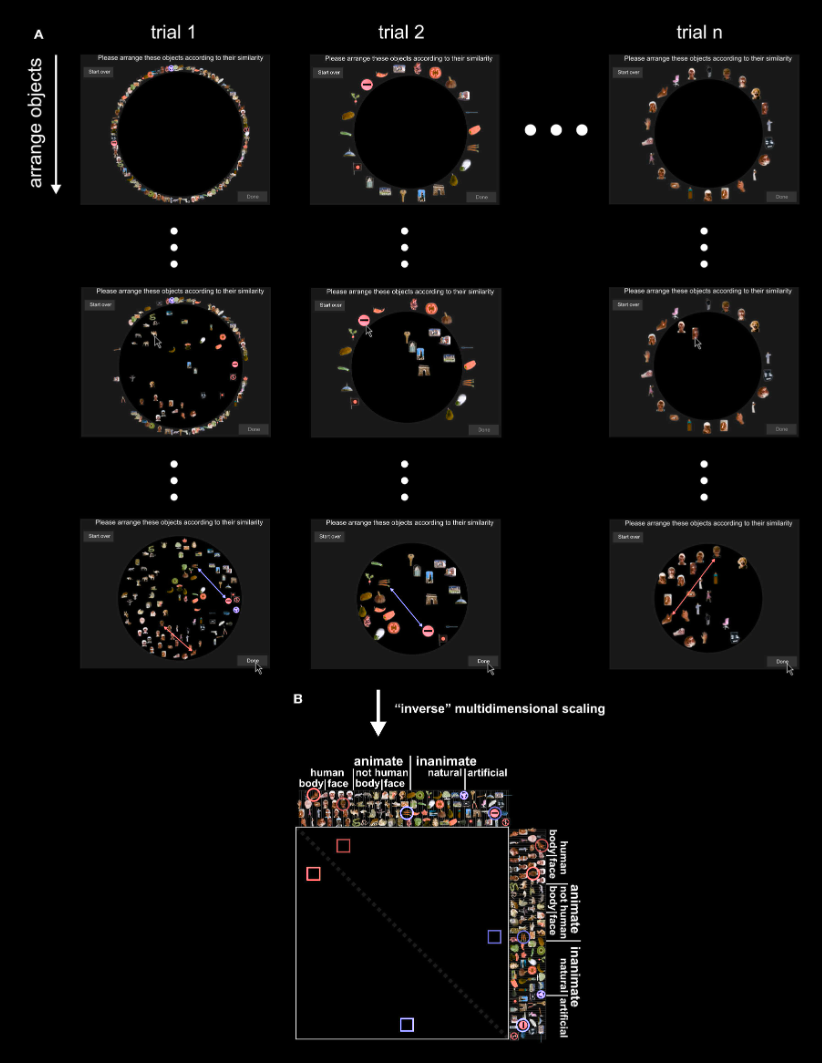
\includegraphics{images/multi-arrangement-method-mur-2013.png}

}

\caption{\label{fig-multi-arrangement}\textbf{Acquiring similarity
judgements with the multi-arrangement method. (A)} Subjects are asked to
arrange items according to their similarity, using mouse drag-and-drop
on a computer. The similarity measure is taken as the distances between
the items: similar items are closer, while dissimilar items are further
apart. The upper part of the figure shows screenshots at different
moments of the acquisition for one subject. Columns are trials and rows
show the object arrangements over time, running from the start (top row)
to the end (last row). The first trial contains all items; subsequent
trials contain subsets of items that are adaptively selected to
optimally estimate judged similarity for each subject. \textbf{(B)} Once
acquisition of the final judgements is completed, inter-item distances
in the final trial arrangements are combined over trials by rescaling
and averaging to yield a single dissimilarity estimate for each object
pair. The process is illustrated in this figure for two example item
pairs: a boy's face and a hand (red), and carrots and a stop sign
(blue). Their single-trial dissimilarity estimates (arrows) are combined
into a single dissimilarity estimate, which is placed at the
corresponding entry of the RDM (lower panel). Mirror-symmetric entries
are indicated by lighter colors. Figure taken from
\citet{murHumanObjectSimilarityJudgments2013}.}

\end{figure}%

A key strength of this method that sets it as particularly effective is
the ``adaptive'' part. The goal of the process is to acquire similarity
judgements as precisely as possible while minimizing the total amount of
trials. To do so, starting from the second trial, selected subsets of
the items to be compared are presented to the subject: these items are
the ones that were very close on-screen in previous trials and thus had
their distance evaluated with lower accuracy by the subject. As the
subject has to fill the entire ``arena'' with the items, these
subsequent trials will necessarily increase the level of precision in
the similarity judgement between pairs of items. The second key benefit
of this method is the time and effort gain compared to others. For
example, to compare every pair of items among 64 different items would
require \(\frac{64 \times (64-1)}{2} = 2016\) comparisons (i.e.~trials).
This would be extremely time-consuming, while also losing the
\emph{context-independence} afforded by the MA method due to the
presence of other items around every time the subject mentally performs
a pairwise comparison.

Historically, when referring to the projection of the representations of
stimuli (e.g., coordinates in geometric space) from a high-dimensional
space into a lower-dimensional space, inference algorithms were commonly
called multidimensional scaling \citep{roads2024}. By analogy, the
process of combining several lower-dimensional (2D) similarity
judgements on-screen to form one higher dimensional similarity
representation (in the RDM) can be conceptually seen as ``inverse''
multidimensional scaling, hence the name given to the method by
\citet{kriegeskorteInverseMDSInferring2012}.

\subsubsection{Principle}\label{principle}

The idea is simple: for a given set of items that have distinct and very
pictorial visual properties, we would ask a wide range of aphantasics,
phantasics or hyperphantasics to imagine, mentally compare and make
similarity judgements between the items. To compare these
representations with actual perceptual representations, the subjects
would also perform the same task afterwards, this time with actual
pictures to compare. Subjects would also fill our usual psychometric
imagery questionnaires.

To ``compare imagined items'', we could use a ``word'' version of the MA
paradigm. An example from
\citet{majewskaSpatialMultiarrangementClustering2020} - \emph{who used
the method to build large-scale semantic similarity resources for
Natural Language Processing systems} - is represented in
Figure~\ref{fig-majewska}.

\begin{figure}

\centering{

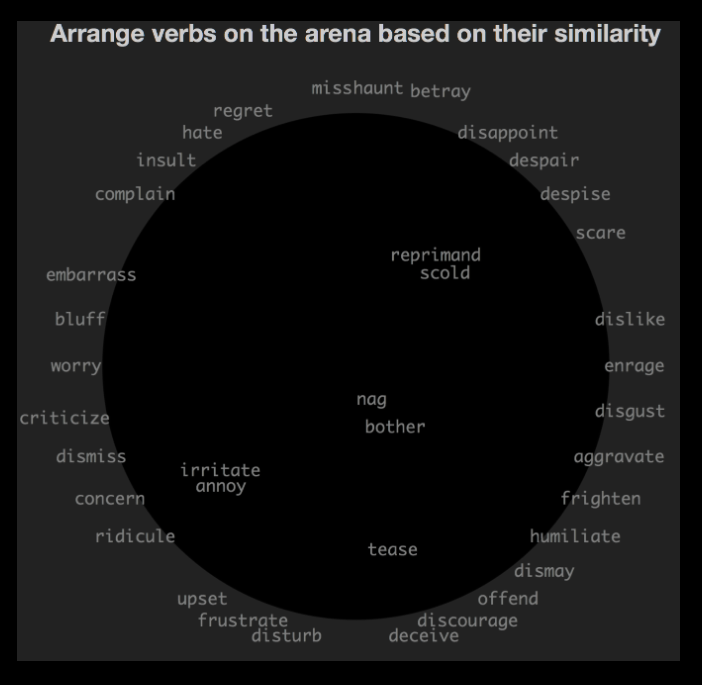
\includegraphics[width=0.5\textwidth,height=\textheight]{images/majewska-spam.png}

}

\caption{\label{fig-majewska}Arena layout of the MA protocol used by
\citet{majewskaSpatialMultiarrangementClustering2020} to acquire
similarity judgements on word pairs.}

\end{figure}%

\subsection{Hypotheses}\label{hypotheses}

\subsubsection{Aphantasic and phantasic psychological
spaces}\label{aphantasic-and-phantasic-psychological-spaces}

The most representative members of a category are called prototypical
members.

Prototype theory builds on the observation that among the instances of a
property, some are more representative than others. The most
representative one is the prototype of the property.

Thus, following the concepts illustrated by Gardenfors, we would expect
that aphantasics, when doing shape similarity judgements, would be more
inclined to group items close to the prototypical items due to a lower
definition of the mental image. In comparison, phantasics would have a
much more distributed conceptual space of item shapes due to their
higher-resolution mental images of said items.

\subsubsection{Subjective imagery and psychological
spaces}\label{subjective-imagery-and-psychological-spaces}

In the proposed view of visual imagery as the subjective expression of a
given type of psychological space, we mentioned earlier that
\emph{spatial} imagery could also constitute a subjective expression of
other dimensions of psychological spaces. Hence, the \emph{verbal}
dimension of the simplified model of imagery we outlined in my thesis
project could also represent different dimensions.

This conception leads to the following theoretical hypothesis: provided
that our visual-spatial-verbal model correctly fits subjective imagery,
the imagery profile of individuals should map on their psychological
spaces.

Operationally, this would be evaluated by the fact that
\textbf{individuals with similar imagery profiles} (visual, spatial,
verbal, or any combination of the three) \textbf{should have similar
representations} in their given psychological space,
\textbf{quantifiable by the degree of alignment between their similarity
structures.}

\begin{figure}[H]

{\centering 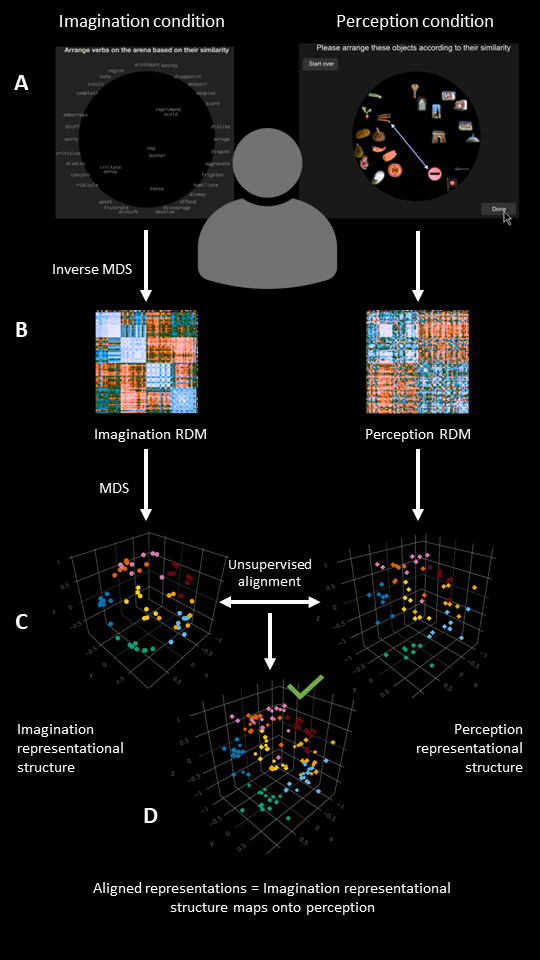
\includegraphics{images/my-protocol-1.png}

}

\caption{The two conditions for one subject.}

\end{figure}%%
\begin{figure}[H]

{\centering 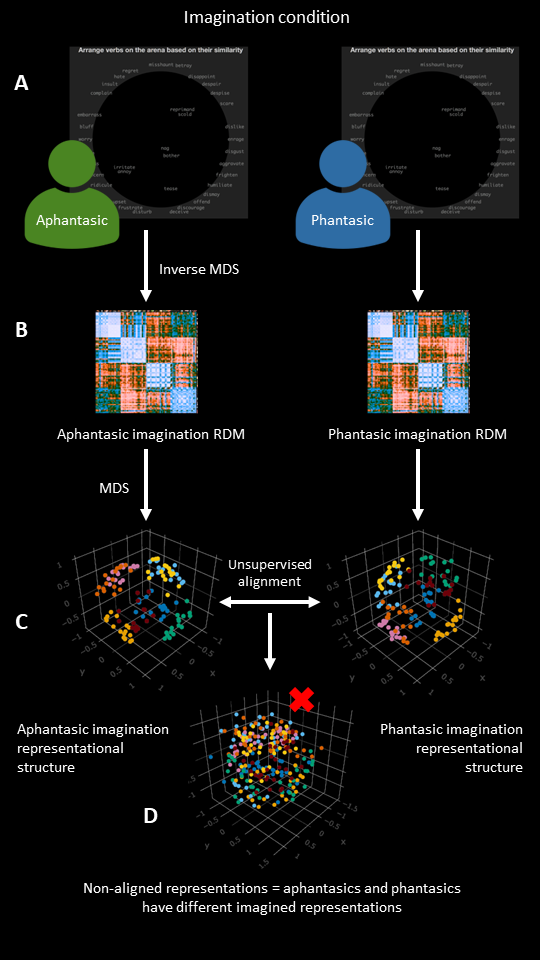
\includegraphics{images/my-protocol-2.png}

}

\caption{The comparison between the representational structure of
aphantasics and phantasics. This figure illustrates the principle, but
in reality all pairs of subjects will be compared to assess their
representational structure alignment. This is computationnally heavy,
but analytically very powerful.}

\end{figure}%

\section{Study data simulation and
analysis}\label{study-data-simulation-and-analysis}

\textsubscript{Source:
\href{https://m-delem.github.io/2499-similarity-manuscript/index.qmd.html}{Article
Notebook}}

\subsection{Visual-spatial-verbal model of cognitive
profiles}\label{visual-spatial-verbal-model-of-cognitive-profiles}

One of the objectives of the study would be to link the subjective
cogntive profiles of individuals with their representational structures.
To evaluate these profiles, we are going to use psychometric
questionnaires evaluating the visual-object, spatial, and verbal
dimensions of imagery which will yield three scores, one for each
dimension.

We are going to simulate 30 participants presenting four different
cognitive profiles, that I defined as, respectively, \emph{verbal}
aphantasics, \emph{spatial} aphantasics, \emph{spatial} phantasics, and
\emph{visual} phantasics. Their imagery abilities are summarised in
Table~\ref{tbl-imageries}.

To simulate these four sub-groups, we use the \texttt{holodeck} R
package to generate multivariate normal distributions of scores on these
three dimensions for each sub-group. For instance, verbal aphantasics
have normally distributed visual imagery scores centered around a mean
of 0 (normalized, so negative scores are possible), 0.4 for spatial
imagery, and 0.7 for verbal style; Spatial aphantasics have means of 0
for visual, 0.75 spatial, and 0.3 for verbal; etc. The numbers are
arbitrary, but have been chosen by trial-and-error to obtain a model
that is both well-defined and not exagerrated. The 30 subjects' imagery
profiles are represented in the three dimensional space of the
visual-spatial-verbal dimensions in Figure~\ref{fig-plot-osv-model}.

\begin{longtable}[]{@{}lccc@{}}
\caption{Imagery abilities of the four hypothesized cognitive
profiles.}\label{tbl-imageries}\tabularnewline
\toprule\noalign{}
Cognitive profile & Visual imagery & Spatial imagery & Verbal style \\
\midrule\noalign{}
\endfirsthead
\toprule\noalign{}
Cognitive profile & Visual imagery & Spatial imagery & Verbal style \\
\midrule\noalign{}
\endhead
\bottomrule\noalign{}
\endlastfoot
Verbal aphantasic & -- & - & ++ \\
Spatial aphantasic & -- & ++ & - \\
Spatial phantasic & + & ++ & - \\
Visual phantasic & ++ & - & + \\
\end{longtable}

Down below is the code to generate these scores.

\begin{Shaded}
\begin{Highlighting}[]
\CommentTok{\# The function takes the variance and covariance of the imagery distributions}
\CommentTok{\# as arguments}
\NormalTok{generate\_osv\_model }\OperatorTok{\textless{}{-}}\NormalTok{ function(var, cov)\{}
\NormalTok{  df }\OperatorTok{\textless{}{-}} 
\NormalTok{    tibble(group }\OperatorTok{=}\NormalTok{ rep(c(}\StringTok{"aph"}\NormalTok{, }\StringTok{"phant"}\NormalTok{), each }\OperatorTok{=} \DecValTok{8}\NormalTok{)) }\OperatorTok{|\textgreater{}} 
\NormalTok{    group\_by(group) }\OperatorTok{|\textgreater{}} 
\NormalTok{    mutate(}
\NormalTok{      spatial\_group }\OperatorTok{=}\NormalTok{ c(rep(}\StringTok{"spa\_low"}\NormalTok{, }\DecValTok{4}\NormalTok{), rep(}\StringTok{"spa\_high"}\NormalTok{, }\DecValTok{4}\NormalTok{)),}
\NormalTok{      vis\_spa\_group }\OperatorTok{=}\NormalTok{ paste0(group, }\StringTok{"\_"}\NormalTok{, spatial\_group),}
\NormalTok{      verbal\_group }\OperatorTok{=} \StringTok{"verbal\_low"}\NormalTok{,}
\NormalTok{      verbal\_group  }\OperatorTok{=}\NormalTok{ case\_when(}
\NormalTok{        vis\_spa\_group }\OperatorTok{==} \StringTok{"aph\_spa\_low"} \OperatorTok{\textasciitilde{}} \StringTok{"verbal\_high"}\NormalTok{, }
\NormalTok{        vis\_spa\_group }\OperatorTok{==} \StringTok{"phant\_spa\_low"} \OperatorTok{\textasciitilde{}} \StringTok{"verbal\_mid"}\NormalTok{,}
\NormalTok{        TRUE }\OperatorTok{\textasciitilde{}}\NormalTok{ verbal\_group)}
\NormalTok{    ) }\OperatorTok{|\textgreater{}} 
\NormalTok{    group\_by(vis\_spa\_group) }\OperatorTok{|\textgreater{}} 
    \CommentTok{\# ─── visual ───}
\NormalTok{    sim\_discr(}
\NormalTok{      n\_vars }\OperatorTok{=} \DecValTok{1}\NormalTok{, }
\NormalTok{      var }\OperatorTok{=}\NormalTok{ var, }
\NormalTok{      cov }\OperatorTok{=}\NormalTok{ cov, }
      \CommentTok{\# aph\_s, aph\_v, phant\_s, phant\_v}
\NormalTok{      group\_means }\OperatorTok{=}\NormalTok{ c(}\DecValTok{0}\NormalTok{, }\DecValTok{0}\NormalTok{, }\FloatTok{0.6}\NormalTok{, }\FloatTok{0.87}\NormalTok{), }
\NormalTok{      name }\OperatorTok{=} \StringTok{"v"}\NormalTok{) }\OperatorTok{|\textgreater{}} 
    \CommentTok{\# ─── spatial ───}
\NormalTok{    sim\_discr(}
\NormalTok{      n\_vars }\OperatorTok{=} \DecValTok{1}\NormalTok{,  }
\NormalTok{      var }\OperatorTok{=}\NormalTok{ var, }
\NormalTok{      cov }\OperatorTok{=}\NormalTok{ cov, }
      \CommentTok{\# aph\_s, aph\_v, phant\_s, phant\_v}
\NormalTok{      group\_means }\OperatorTok{=}\NormalTok{ c(}\FloatTok{0.75}\NormalTok{, }\FloatTok{0.4}\NormalTok{, }\FloatTok{0.7}\NormalTok{, }\FloatTok{0.3}\NormalTok{), }
\NormalTok{      name }\OperatorTok{=} \StringTok{"s"}\NormalTok{) }\OperatorTok{|\textgreater{}}
    \CommentTok{\# ─── verbal ───}
\NormalTok{    sim\_discr(}
\NormalTok{      n\_vars }\OperatorTok{=} \DecValTok{1}\NormalTok{,  }
\NormalTok{      var }\OperatorTok{=}\NormalTok{ var, }
\NormalTok{      cov }\OperatorTok{=}\NormalTok{ cov, }
      \CommentTok{\# aph\_s, aph\_v, phant\_s, phant\_v}
\NormalTok{      group\_means }\OperatorTok{=}\NormalTok{ c(}\FloatTok{0.3}\NormalTok{, }\FloatTok{0.7}\NormalTok{, }\FloatTok{0.3}\NormalTok{, }\FloatTok{0.5}\NormalTok{), }
\NormalTok{      name }\OperatorTok{=} \StringTok{"i"}\NormalTok{) }\OperatorTok{|\textgreater{}}
\NormalTok{    rename(}
\NormalTok{      visual\_imagery  }\OperatorTok{=}\NormalTok{ v\_1,}
\NormalTok{      spatial\_imagery }\OperatorTok{=}\NormalTok{ s\_1,}
\NormalTok{      verbal\_profile  }\OperatorTok{=}\NormalTok{ i\_1}
\NormalTok{      )}
\NormalTok{\}}

\NormalTok{df }\OperatorTok{\textless{}{-}}\NormalTok{ generate\_osv\_model(}\FloatTok{0.03}\NormalTok{, }\DecValTok{0}\NormalTok{)}
\end{Highlighting}
\end{Shaded}

\textsubscript{Source:
\href{https://m-delem.github.io/2499-similarity-manuscript/notebooks/simulation-code-preview.html\#cell-osv-model}{Simulation
code}}

\phantomsection\label{cell-fig-plot-osv-model}
\begin{figure}[H]

\centering{

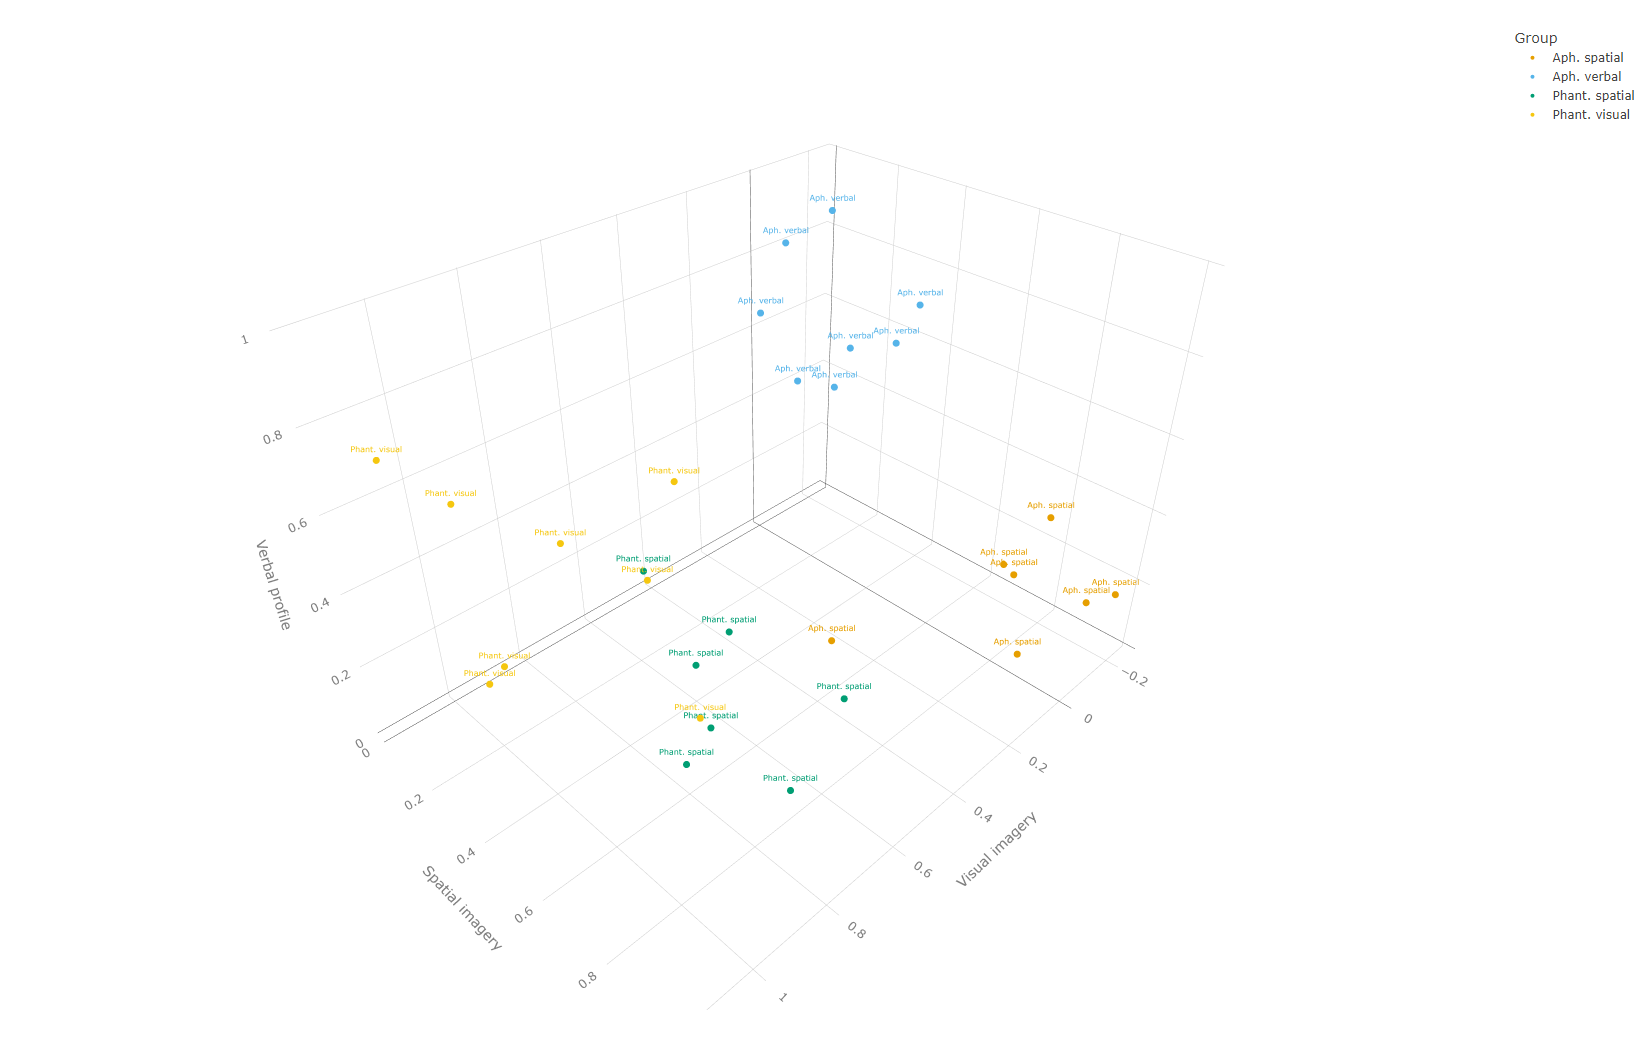
\includegraphics{index_files/figure-pdf/fig-plot-osv-model-1.png}

}

\caption{\label{fig-plot-osv-model}Imagery profiles generated for 30
subjects on the three object, spatial, and verbal dimensions.}

\end{figure}%

\textsubscript{Source:
\href{https://m-delem.github.io/2499-similarity-manuscript/index.qmd.html}{Article
Notebook}}


  \bibliography{references.bib}


\end{document}
